\documentclass[page number,dvipsnames]{beamer}
\usetheme[sectionpage=none,numbering=fraction,progressbar=foot]{metropolis}

\usepackage{pgf,tikz}
\usetikzlibrary{arrows}
\usetikzlibrary{positioning,shapes,fit}
\usepackage{xcolor}
\usepackage{amssymb}
\usepackage{amsmath}
\usepackage{url}
\usepackage{listings}
\usepackage{lstcoq}


\makeatletter
\makeatother

\setcounter{tocdepth}{1} % remove subsection from table of contents

% colors
\definecolor{mDarkRed}{HTML}{6F1616}
\definecolor{mDarkGreen}{HTML}{106235}
\definecolor{mTeal}{HTML}{112233}
\definecolor{mBlack}{HTML}{000000}
\setbeamercolor{normal text}{fg=mTeal}
\setbeamercolor{alerted text}{fg=mDarkRed}
\setbeamercolor{example text}{fg=mDarkGreen}
\setbeamercolor{title separator}{fg=purple,bg=mBlack}

\definecolor{spec}{HTML}{6F1616}
\definecolor{prog}{HTML}{106235}


\lstset{language=[Objective]{Caml},
                basicstyle=\ttfamily\tiny,
                keywordstyle=\color{RedViolet}\ttfamily,
                stringstyle=\color{Violet}\ttfamily,
                commentstyle=\color{MidnightBlue}\ttfamily,
                morecomment=[l][\color{magenta}]{\#},
                morekeywords={bool, list, int},
                emph={%  
                  Inductive, Lemma%
                },emphstyle={\color{Maroon}}
}

\def\outline{
  \begin{frame}[plain,noframenumbering]
    \frametitle{Outline}
    \tableofcontents[currentsection]
  \end{frame}
}


\begin{document}
\title[Pretty Big Step]{Pretty-Big-Step Semantics}

\author[Aur\`ele Barri\`ere]{Aur\`ele Barri\`ere}

\date{\textbf{December 7, 2018}}

\def\outline{
  \begin{frame}[plain,noframenumbering]
    \frametitle{Outline}
    \tableofcontents[currentsection]
  \end{frame}
}

\begin{frame}[plain,noframenumbering]
  \vspace{-2cm}
  \maketitle
  \vspace{-4cm}
\end{frame}

%% \metroset{sectionpage=none}

%% \metroset{sectionpage=progressbar}

\begin{frame}{Pretty-Big-Step Semantics}
  \begin{itemize}
  \item Operational Semantics.
  \item Inspired by Big-Step Semantics.
  \item Choosing a Semantics' style is about the way of writing the rules and doing the proofs, not expressivity.
  \end{itemize}
  \vfill
  \begin{alertblock}{Small-Step Semantics}
    Step: $(\mathit{code},\mathit{State})\rightarrow(\mathit{code},\mathit{State})$.\\
    Many steps until final configuration.
  \end{alertblock}
  \vfill
  \begin{exampleblock}{Big-Step Semantics}
    One step: $(\mathit{code},\mathit{State})\rightarrow\mathit{State}$.
  \end{exampleblock}
  
\end{frame}

\begin{frame}{Small-step Reminder}
  \center
  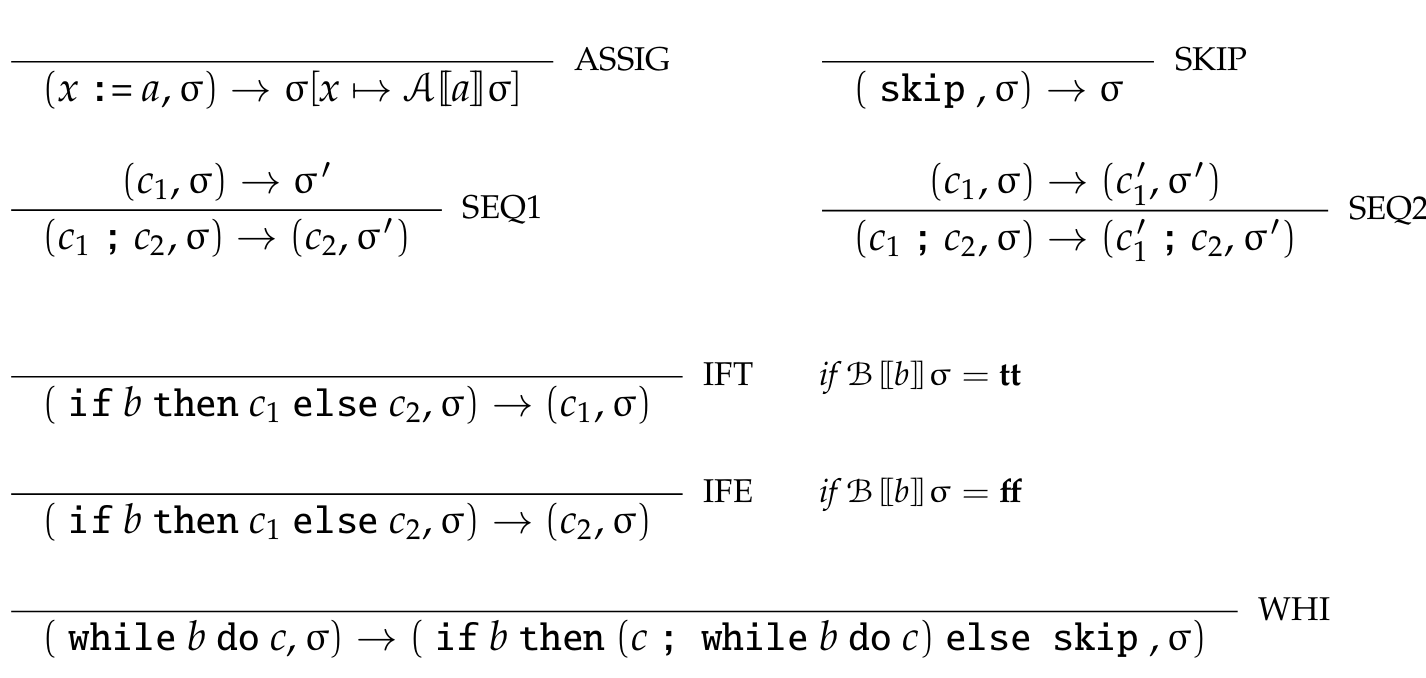
\includegraphics[scale=0.2]{smallstep.png}
\end{frame}

\begin{frame}{Big-step Reminder}
  \center
  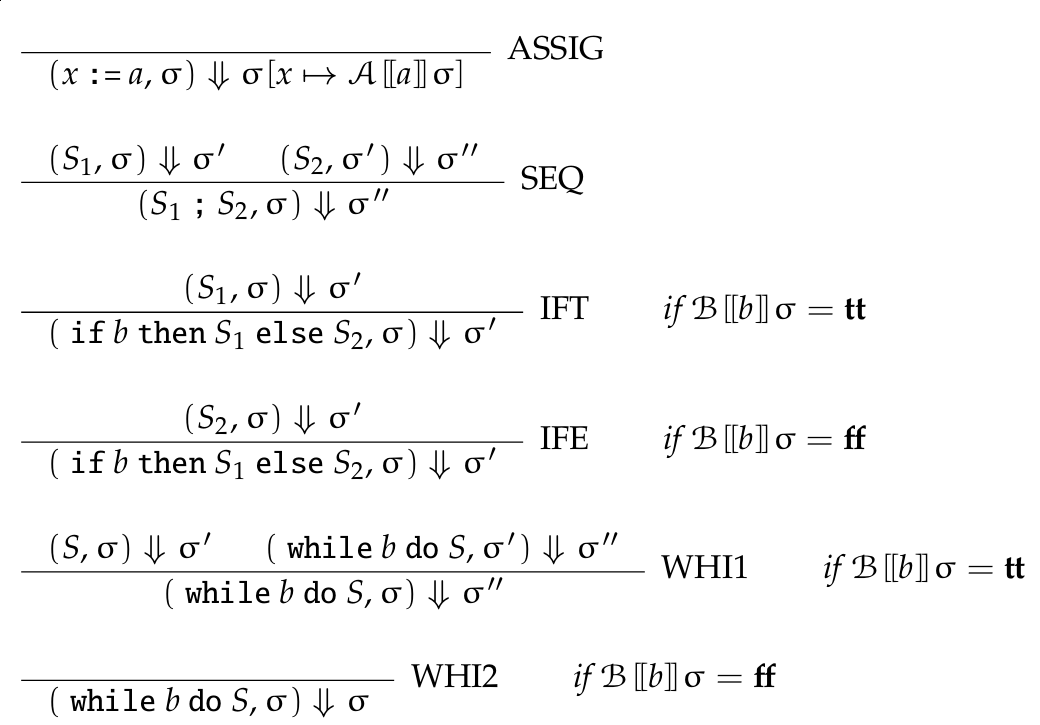
\includegraphics[scale=0.2]{bigstep.png}
\end{frame}


\begin{frame}{Why Pretty-Big-Step Semantics?}
  \begin{block}{Big-Step is still used}
    \begin{itemize}
    \item 17 out of 40 operational semantics in recent conferences.
    \item Cost semantics, informal description.
    \item Some proofs need to be done on big-step semantics.
    \end{itemize}
  \end{block}
  \vfill
  \begin{alertblock}{Drawbacks of Big-Step Semantics}
    Redundancy when adding new constructs.\\
    For instance: divergence, errors, control-flow exceptions\dots
  \end{alertblock}
\end{frame}

\begin{frame}{Duplicating rules in Big-Step Semantics}
  The example of divergent behavior.\\
  \center
  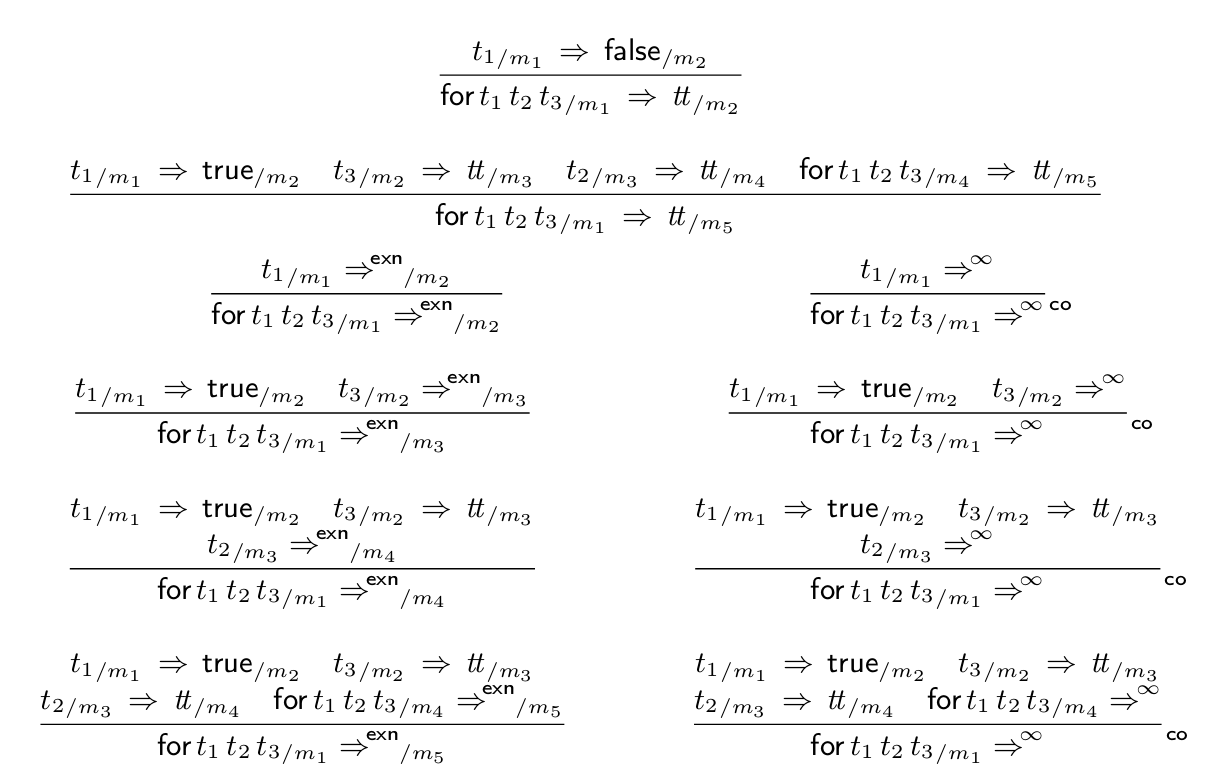
\includegraphics[scale=0.25]{duplicates.png}
  
\end{frame}

\begin{frame}{Pretty-Big Step Presentation}
  \begin{exampleblock}{Properties}
    \begin{itemize}
    \item less rules.
    \item no duplication of premises.
    \item use coinduction for diverging behaviors.
    \item add intermediate terms
    \end{itemize}
  \end{exampleblock}
  \vfill
  \begin{block}{Example: $\lambda$-calculus}
    \center
    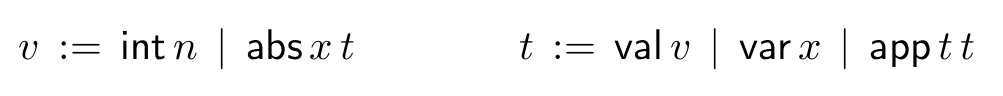
\includegraphics[scale=0.3]{lambda.png}
  \end{block}
\end{frame}

\begin{frame}{Evaluating Application}
  \begin{alertblock}{Big-Step}
    \center
    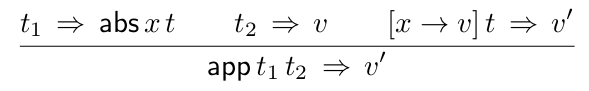
\includegraphics[scale=0.3]{bigstep_betared.png}
  \end{alertblock}
  \vfill
  \begin{block}{First Attempt at Pretty-Big-Step}
    \center
    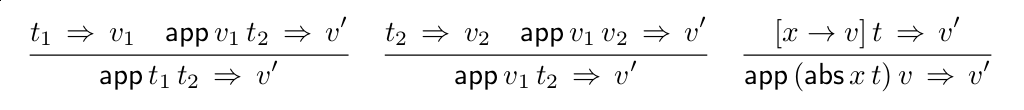
\includegraphics[scale=0.3]{first_attempt_betared.png}
  \end{block}
  \begin{alertblock}{Overlapping Problem}
    Evaluation isn't syntax-directed.
  \end{alertblock}
\end{frame}

\begin{frame}{Intermediate Terms}
  \begin{block}{Term Syntax}
    \center
    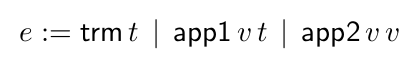
\includegraphics[scale=0.3]{interm.png}
  \end{block}
  \vfill
  \begin{exampleblock}{Non-overlapping Semantics}
    \center
    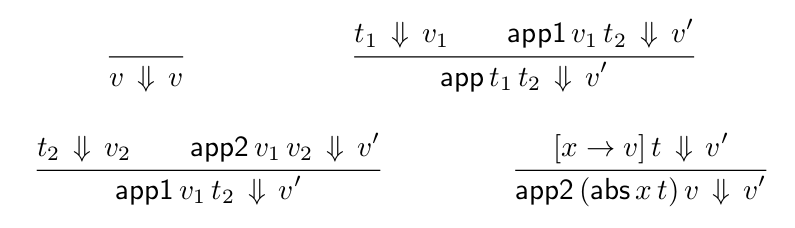
\includegraphics[scale=0.3]{interm_step.png}
  \end{exampleblock}
\end{frame}

\def\app{\mathbf{app}}
\def\abs{\mathbf{abs}}
\begin{frame}{Example}
  Evaluation of $(\lambda y.~ (y ~0))~ (\lambda x.~ x + 2)$.\\
  $\app~(\abs~ y~ (\app~ y~ 0))~(\abs~ x~ (x+2)))$.
  \vfill
\end{frame}


\begin{frame}{Exceptions}
  \begin{block}{Generalized Behavior and Extended Intermediate Terms}
    \begin{center}
    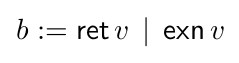
\includegraphics[scale=0.3]{behavior.png}\hfill
    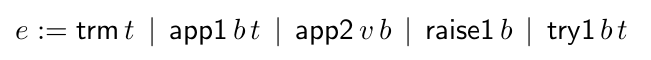
\includegraphics[scale=0.3]{expr_ex.png}
    \end{center}
  \end{block}
  \vfill
  \begin{exampleblock}{Pretty-Big-Step Rules}
    \center
    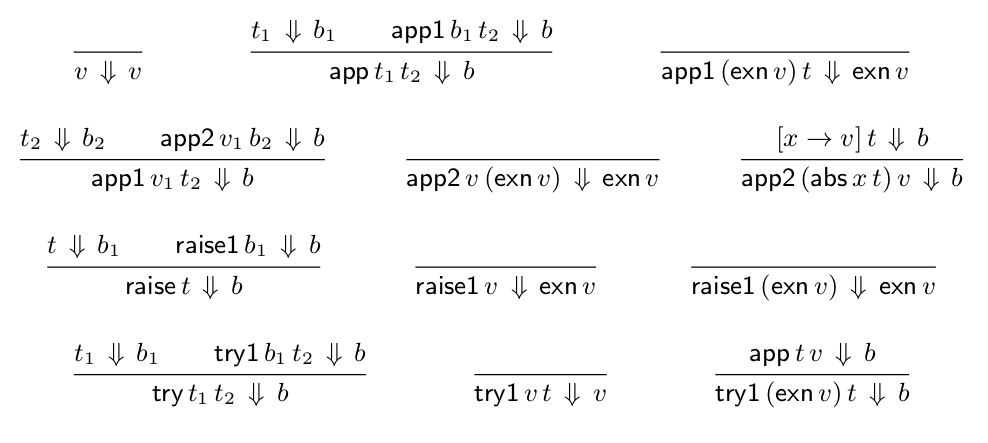
\includegraphics[scale=0.3]{ex_rules.png}
  \end{exampleblock}
\end{frame}

\begin{frame}{Divergence}
  \center
  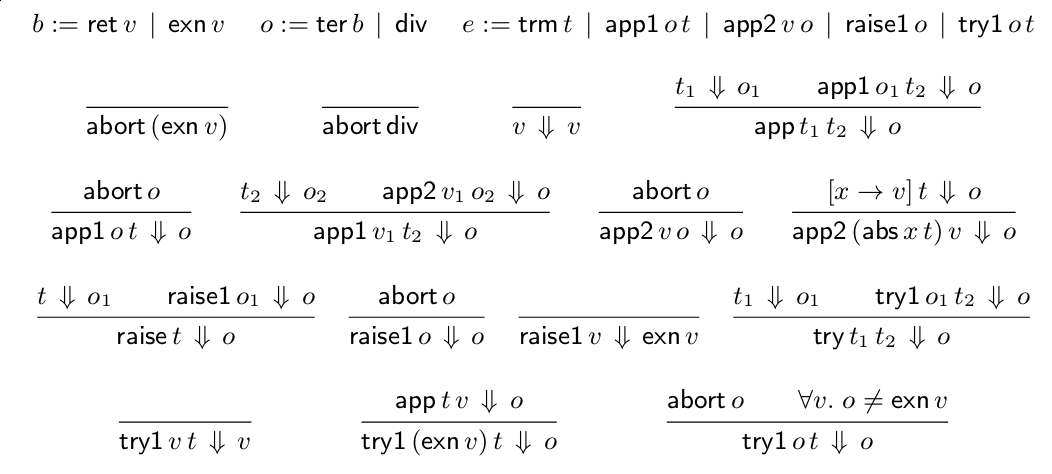
\includegraphics[scale=0.3]{div_rules.png}
\end{frame}

\begin{frame}[fragile]{Coinduction}
  \begin{lstlisting}[language=Coq]
Section stream.
  Variable A : Type.

CoInductive stream : Type :=
  | Cons : A -> stream -> stream.
End stream.
  \end{lstlisting}
  \vfill
  \begin{alertblock}{Guardedness Condition}
    Every co-recursive call must be guarded by a constructor.
  \end{alertblock}
  \vfill
  \url{http://adam.chlipala.net/cpdt/html/Coinductive.html}
\end{frame}

\begin{frame}{Properties}
  \center
  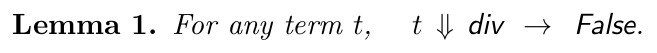
\includegraphics[scale=0.3]{lemma1.png}
  \vfill
  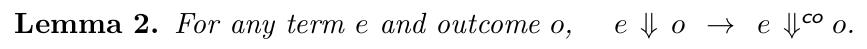
\includegraphics[scale=0.3]{lemma2.png}
  \vfill
  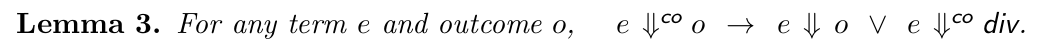
\includegraphics[scale=0.3]{lemma3.png}
  \vfill
  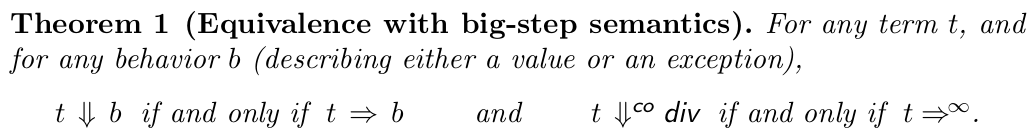
\includegraphics[scale=0.3]{thm1.png}
  \vfill
  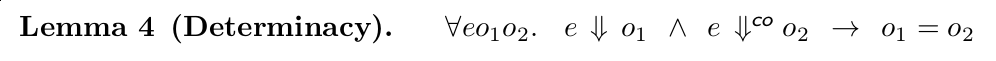
\includegraphics[scale=0.3]{lemma4.png}
\end{frame}

\begin{frame}{Errors and Tying Soundness}
  \begin{block}{Generic Error Rule}
    \center
    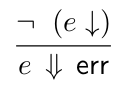
\includegraphics[scale=0.3]{error.png}
  \end{block}
  \vfill
  \begin{exampleblock}{Type Soundness}
    \center
    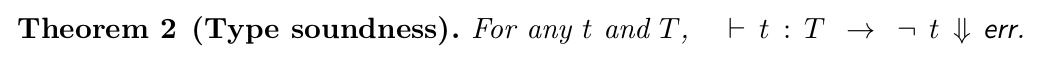
\includegraphics[scale=0.3]{thm2.png}
  \end{exampleblock}
\end{frame}

\begin{frame}{Traces}
  \center
  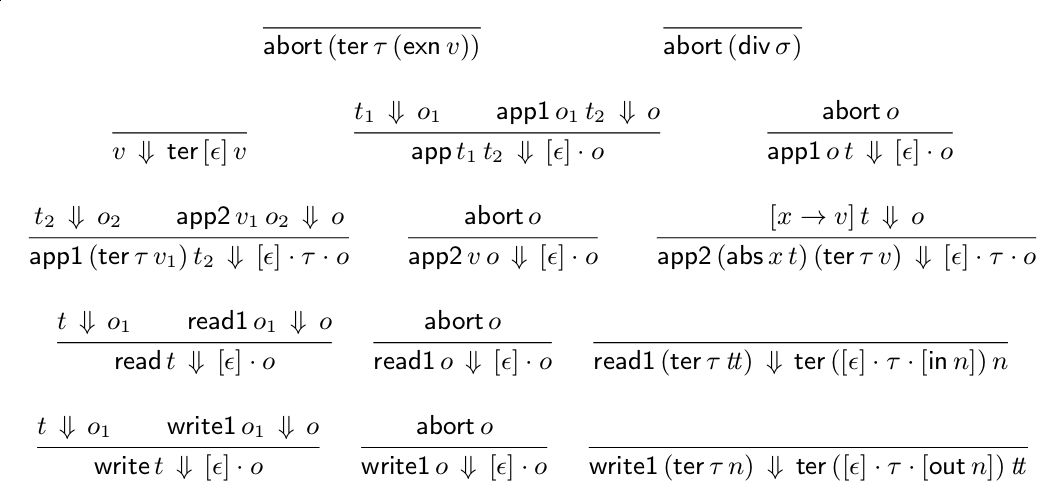
\includegraphics[scale=0.25]{traces.png}
  \vfill
  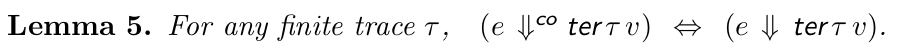
\includegraphics[scale=0.3]{lemma5.png}
\end{frame}

\begin{frame}{Scaling Up}
  \begin{block}{Side-effects}
    \center
    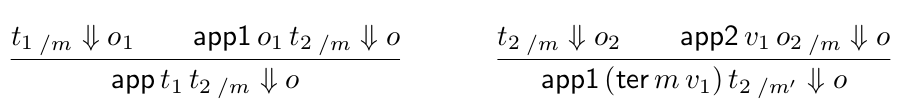
\includegraphics[scale=0.3]{side_effect.png}
  \end{block}
  \vfill
  \begin{block}{Other Functionalities}
    \begin{itemize}
    \item For Loops
    \item Tuples
    \item Generic Abort Rule
    \end{itemize}
  \end{block}

\end{frame}

\begin{frame}{Formalization of core-Caml}
  \begin{exampleblock}{Features}
    \begin{itemize}
    \item Booleans, Integers, Tuples, Algebraic Data Types, records
    \item Functions, Recursive functions, applications, sequences
    \item Conditionals, for loops, while loops
    \item Pattern-matching, let-bindings, assertions
    \end{itemize}
  \end{exampleblock}
  \vfill
  \begin{alertblock}{Missing Features}
    \begin{itemize}
    \item Floats
    \item Mutual Recursion
    \item With construct for records
    \item Arrays
    \item Objects, Modules
    \end{itemize}
  \end{alertblock}

\end{frame}

\begin{frame}[fragile]{Formalization of core-Caml}
  \begin{center}
    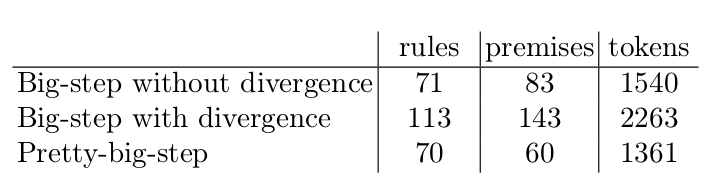
\includegraphics[scale=0.3]{tokens.png}
  \end{center}
  \vfill
  \begin{lstlisting}
(** Grammar of outcomes *)
Inductive out :=
  | out_beh : mem -> beh -> out
  | out_div : out.

(** Grammar of extended terms *)
Inductive ext : Type :=
  | ext_trm : trm -> ext
  | ext_binary_1 : prim -> out -> trm -> ext
  | ext_binary_2 : prim -> val -> out -> ext
  | ext_app_1 : out -> trm -> ext
  ...

Lemma soundness : forall t T, 
  typing empty t T -> ~ red t out_err.
  \end{lstlisting}
  \vfill
  \url{http://www.chargueraud.org/research/2012/pretty/}
\end{frame}

\begin{frame}{Overview}
  European Symposium of Programming, 2013. 43 citations.
  \vfill
  \begin{exampleblock}{Further Works}
    \begin{itemize}
    \item A trusted mechanized JavaScript specification, 2014
    \item Certified Abstract Interpretation with Pretty-Big-Step Semantics, 2015
    \item Functional Big-Step Semantics, 2016
    \end{itemize}
  \end{exampleblock}
  \vfill
  \begin{alertblock}{Questions}
    \begin{itemize}
    \item Determinacy lemma?
    \item What's specific to Pretty-Big-Step?
    \item Typing Complexity?
    \item Standard notion of Coinduction.
    \end{itemize}
  \end{alertblock}

\end{frame}

\begin{frame}{Conclusion}
  \begin{itemize}
  \item New operational Semantics.
  \item Inspired by and Equivalent to Big-Step.
  \item Less rules, more factorization.
  \item Adding functionalities is easier.
  \item Implemented a full language (core-Ocaml).
  \item Size reduction of 40\%.
  \item Co-Inductive proofs cannot be done in Coq yet.
  \end{itemize}
\end{frame}

\end{document}
